% Digital Logic Report Template
% Created: 2020-01-10, John Miller

%==========================================================
%=========== Document Setup  ==============================

% Formatting defined by class file
\documentclass[11pt]{article}

% ---- Document formatting ----
\usepackage[margin=1in]{geometry}	% Narrower margins
\usepackage{booktabs}				% Nice formatting of tables
\usepackage{graphicx}				% Ability to include graphics

%\setlength\parindent{0pt}	% Do not indent first line of paragraphs 
\usepackage[parfill]{parskip}		% Line space b/w paragraphs
%	parfill option prevents last line of pgrph from being fully justified

% Parskip package adds too much space around titles, fix with this
\RequirePackage{titlesec}
\titlespacing\section{0pt}{8pt plus 4pt minus 2pt}{3pt plus 2pt minus 2pt}
\titlespacing\subsection{0pt}{4pt plus 4pt minus 2pt}{-2pt plus 2pt minus 2pt}
\titlespacing\subsubsection{0pt}{2pt plus 4pt minus 2pt}{-6pt plus 2pt minus 2pt}

% ---- Hyperlinks ----
\usepackage[colorlinks=true,urlcolor=blue]{hyperref}	% For URL's. Automatically links internal references.

% ---- Code listings ----
\usepackage{listings} 					% Nice code layout and inclusion
\usepackage[usenames,dvipsnames]{xcolor}	% Colors (needs to be defined before using colors)

% Define custom colors for listings
\definecolor{listinggray}{gray}{0.98}		% Listings background color
\definecolor{rulegray}{gray}{0.7}			% Listings rule/frame color

% Style for Verilog
\lstdefinestyle{Verilog}{
	language=Verilog,					% Verilog
	backgroundcolor=\color{listinggray},	% light gray background
	rulecolor=\color{blue}, 			% blue frame lines
	frame=tb,							% lines above & below
	linewidth=\columnwidth, 			% set line width
	basicstyle=\small\ttfamily,	% basic font style that is used for the code	
	breaklines=true, 					% allow breaking across columns/pages
	tabsize=3,							% set tab size
	commentstyle=\color{gray},	% comments in italic 
	stringstyle=\upshape,				% strings are printed in normal font
	showspaces=false,					% don't underscore spaces
}

% How to use: \Verilog[listing_options]{file}
\newcommand{\Verilog}[2][]{%
	\lstinputlisting[style=Verilog,#1]{#2}
}




%======================================================
%=========== Body  ====================================
\begin{document}

\title{ELC 2137 Lab 11: FSM: Guessing Game}
\author{Alexander Noll}

\maketitle


\section*{Summary}

In this lab a small game of chance was created using a finite state machine(FSM) and a Basys3 board. In order to make the game run better, debouncing was coded for each button input as a way of stabilization. Two different mode of the game were formed by allowing to player to chose between two different play speeds. The object of the game was to press the button corresponding to the currently lit segment on the display. since the normal clock moves degrees higher than a human eye can see, it becomes a game of chance. The clock is slowed to a visible yet fast rate for the easier mode.


\section*{Q\&A}
\begin{enumerate}
	\item wait1= 220ns; one=245ns; wait0=620ns; zero=645ns; Twait=25ns.
	\item Because the next course of action depends what state the system is in.
	\item I utilized a Moore machine as the output (y) was defined within each state.
\end{enumerate}



\clearpage

\section*{Results}

\begin{table*}[ht]\centering
	\caption{\textit{register} Test Results: Fast Mode = (3/10) Success Rate; Slow Mode = 1/2 Success Rate }
	\label{TestResult}\medskip
	\begin{tabular}{l|rrrrrrrrrr}
		Test: 		& 1 & 2 & 3 & 4 & 5 & 6 & 7 & 8 & 9 & 10 \\
		\midrule
		Fast Mode   & lose & win & lose & lose  & lose & win & lose & lose & lose & win \\
		Segment   & bottom & bottom & bottom & top & top & left & left & bottom & right & top \\
		Slow Mode  	& win & lose & win & lose & lose & win & lose & lose & win & win \\
		Segment   & top & left & bottom & left & top & right & right & top & top & bottom \\
		\bottomrule
	\end{tabular}
\end{table*}

\subsection{Test Photos}

\begin{figure}[ht]\centering
	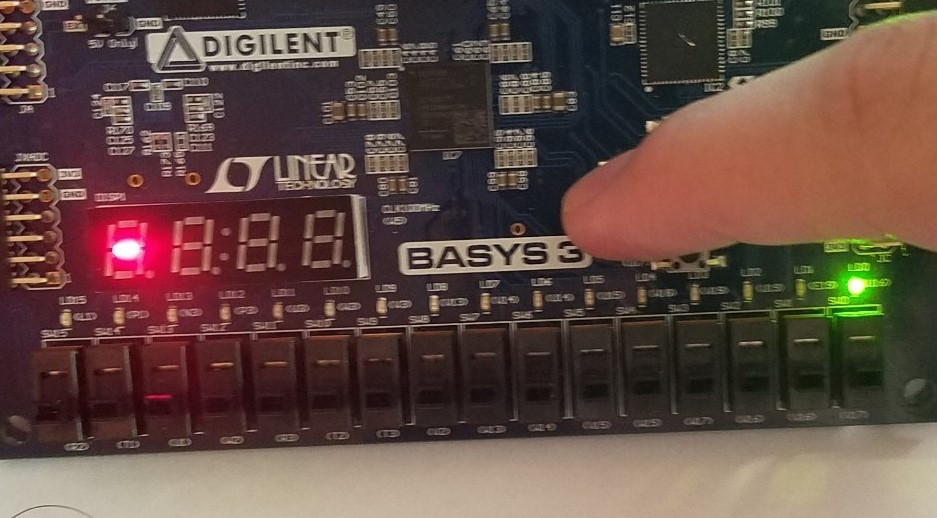
\includegraphics[width=1.0\textwidth,trim=0 0mm 0 0,clip]{Fast1}
	\caption{Fast Mode Test 1}
\end{figure}
\begin{figure}[ht]\centering
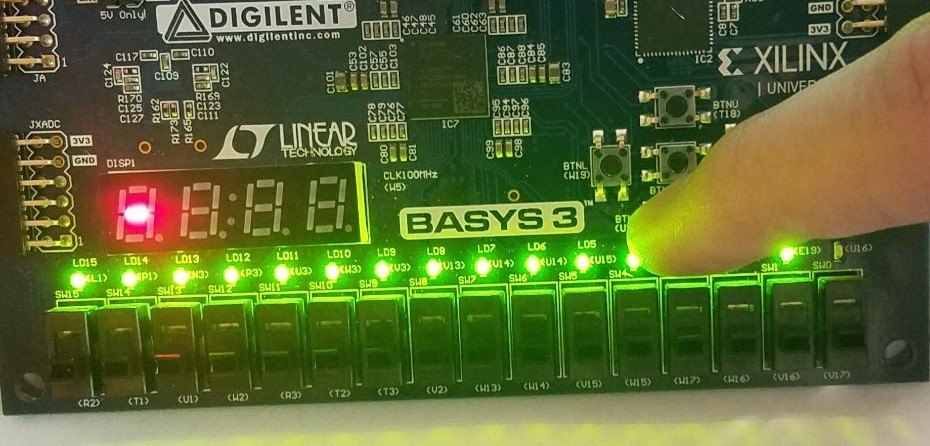
\includegraphics[width=1.0\textwidth,trim=0 0mm 0 0,clip]{Fast2}
\caption{Fast Mode Test 2}
\end{figure}
\begin{figure}[ht]\centering
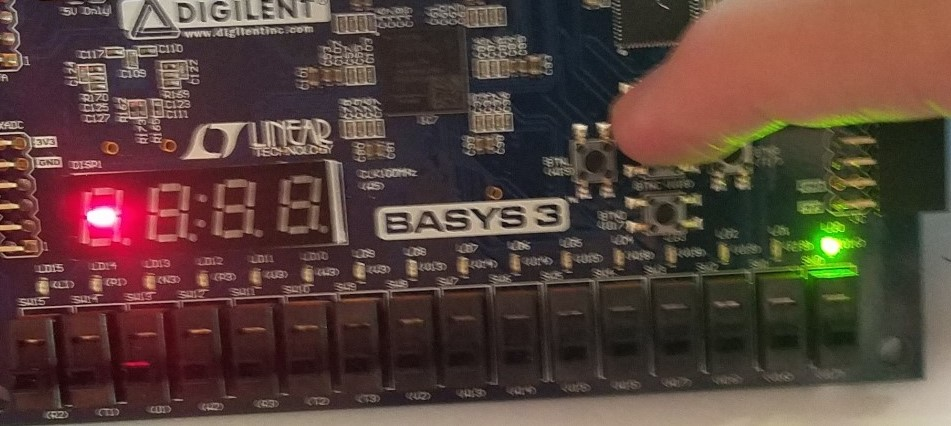
\includegraphics[width=1.0\textwidth,trim=0 0mm 0 0,clip]{Fast3}
\caption{Fast Mode Test 3}
\end{figure}
\begin{figure}[ht]\centering
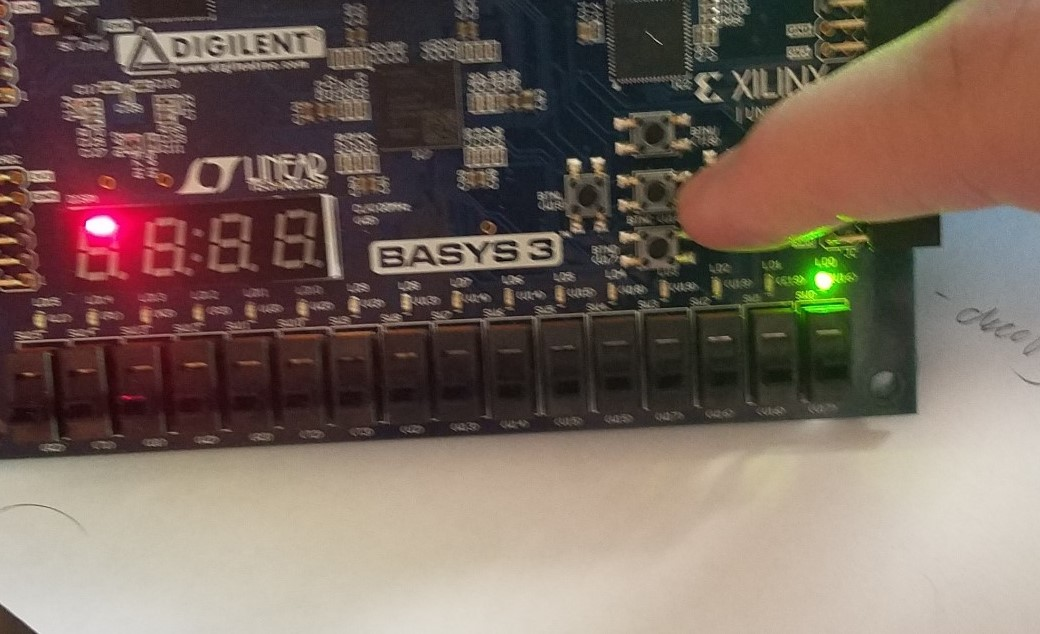
\includegraphics[width=1.0\textwidth,trim=0 0mm 0 0,clip]{Fast4}
\caption{Fast Mode Test 4}
\end{figure}
\begin{figure}[ht]\centering
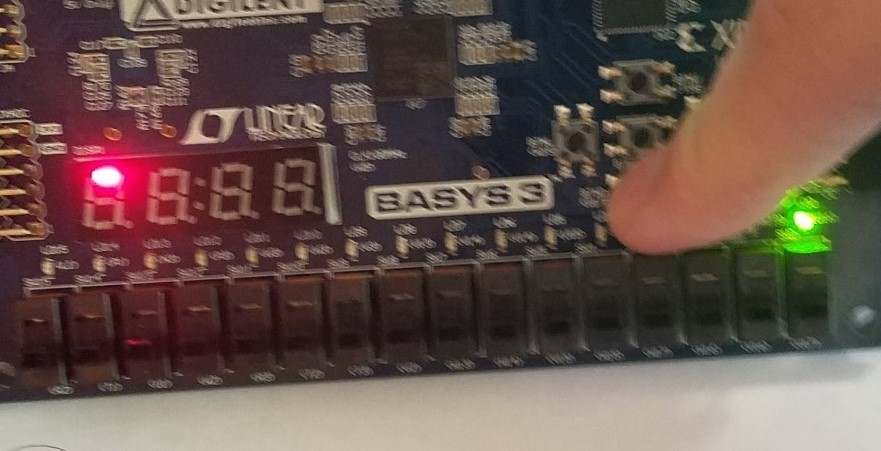
\includegraphics[width=1.0\textwidth,trim=0 0mm 0 0,clip]{Fast5}
\caption{Fast Mode Test 5}
\end{figure}
\begin{figure}[ht]\centering
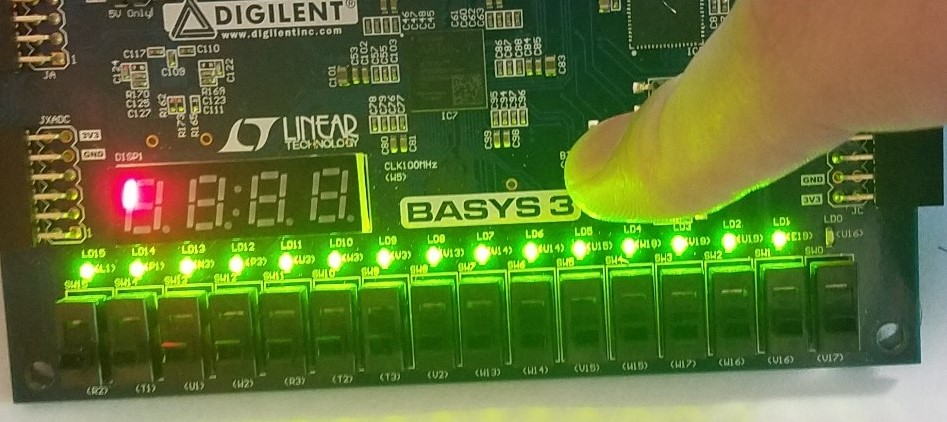
\includegraphics[width=1.0\textwidth,trim=0 0mm 0 0,clip]{Fast6}
\caption{Fast Mode Test 6}
\end{figure}
\begin{figure}[ht]\centering
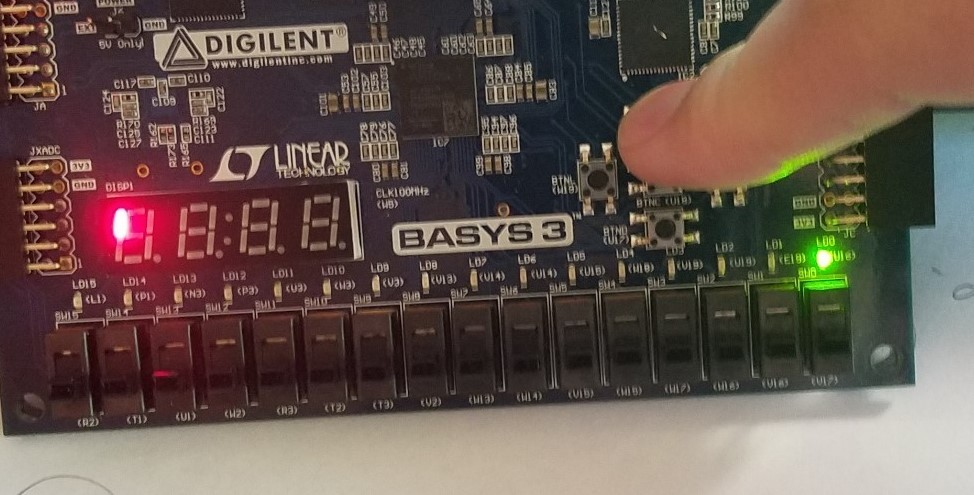
\includegraphics[width=1.0\textwidth,trim=0 0mm 0 0,clip]{Fast7}
\caption{Fast Mode Test 7}
\end{figure}
\begin{figure}[ht]\centering
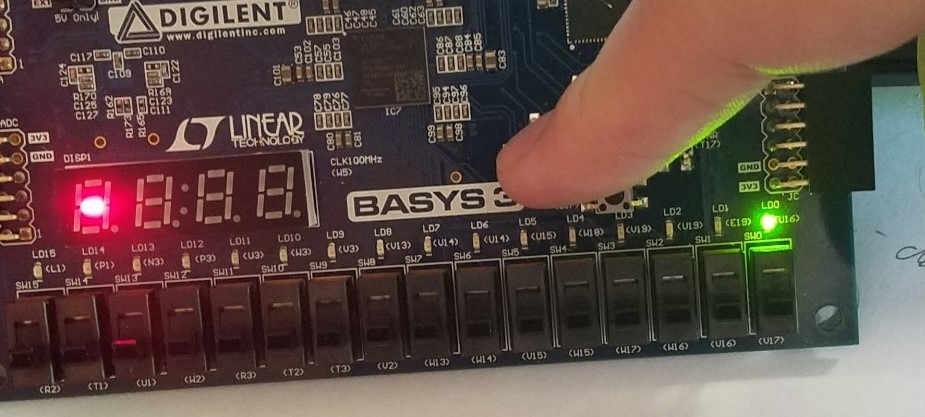
\includegraphics[width=1.0\textwidth,trim=0 0mm 0 0,clip]{Fast8}
\caption{Fast Mode Test 8}
\end{figure}
\begin{figure}[ht]\centering
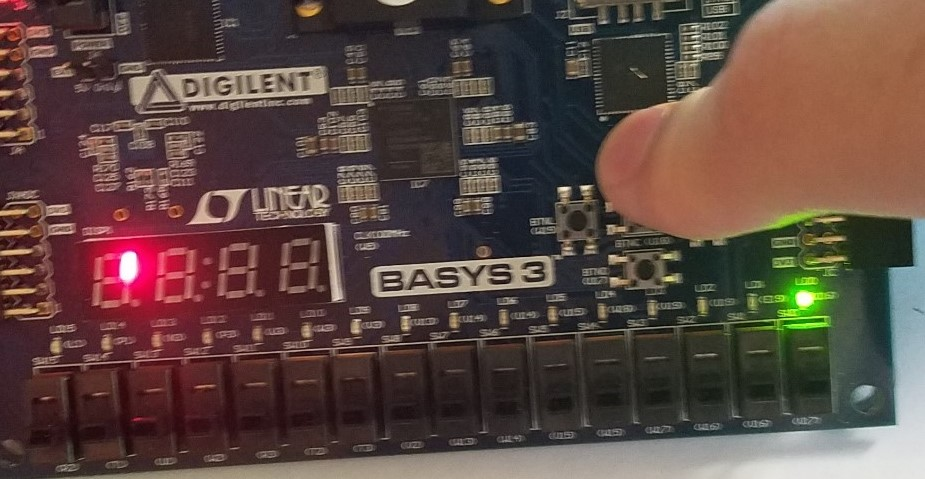
\includegraphics[width=1.0\textwidth,trim=0 0mm 0 0,clip]{Fast9}
\caption{Fast Mode Test 9}
\end{figure}
\begin{figure}[ht]\centering
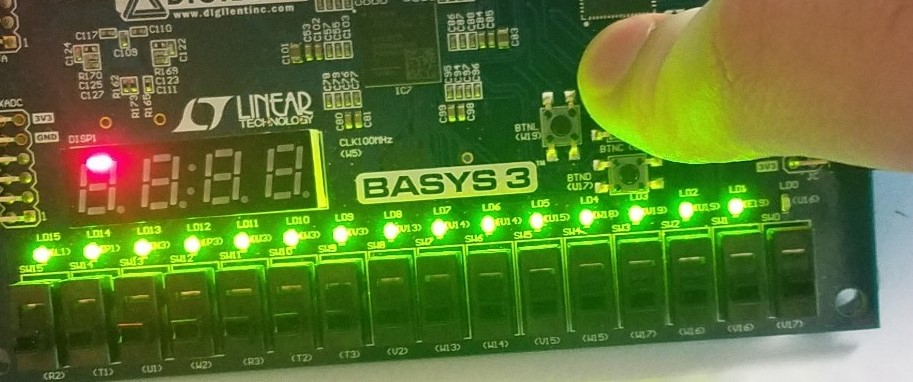
\includegraphics[width=1.0\textwidth,trim=0 0mm 0 0,clip]{Fast10}
\caption{Fast Mode Test 10}
\end{figure}


\begin{figure}[ht]\centering
	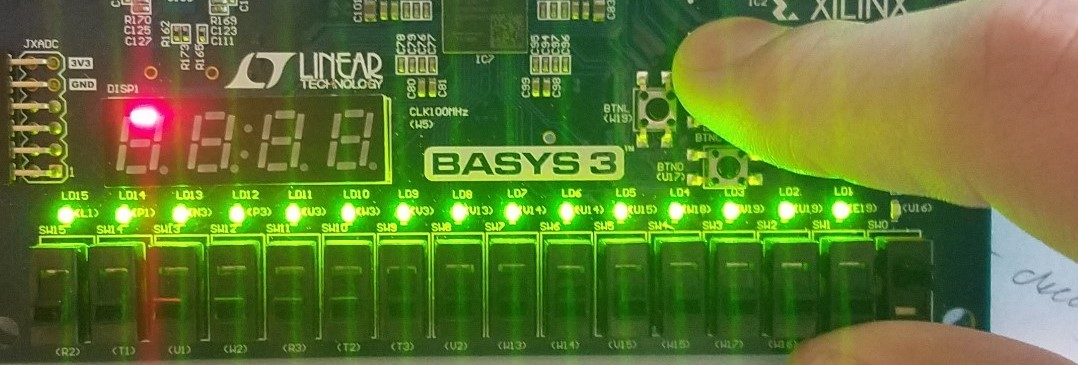
\includegraphics[width=1.0\textwidth,trim=0 0mm 0 0,clip]{Slow1}
	\caption{Slow Mode Test 1}
\end{figure}
\begin{figure}[ht]\centering
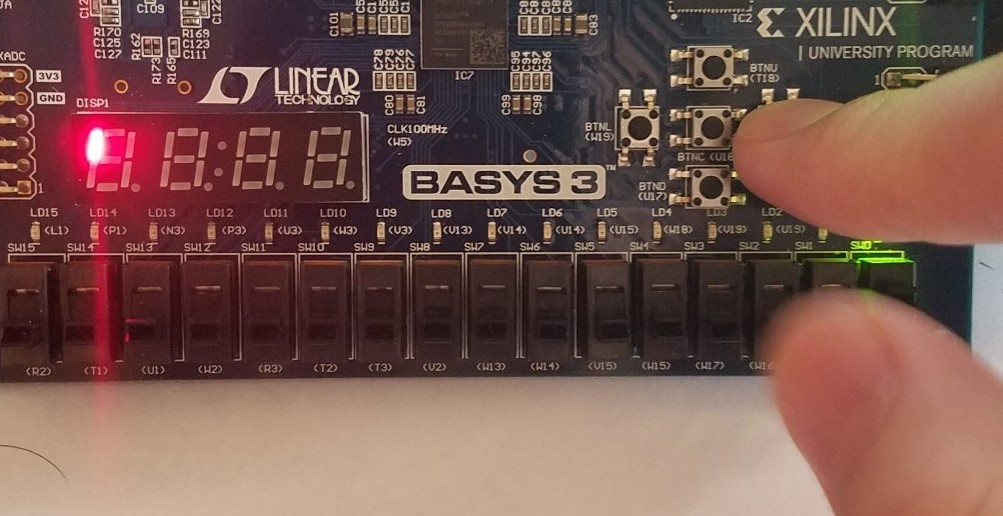
\includegraphics[width=1.0\textwidth,trim=0 0mm 0 0,clip]{Slow2}
\caption{Slow Mode Test 2}
\end{figure}
\begin{figure}[ht]\centering
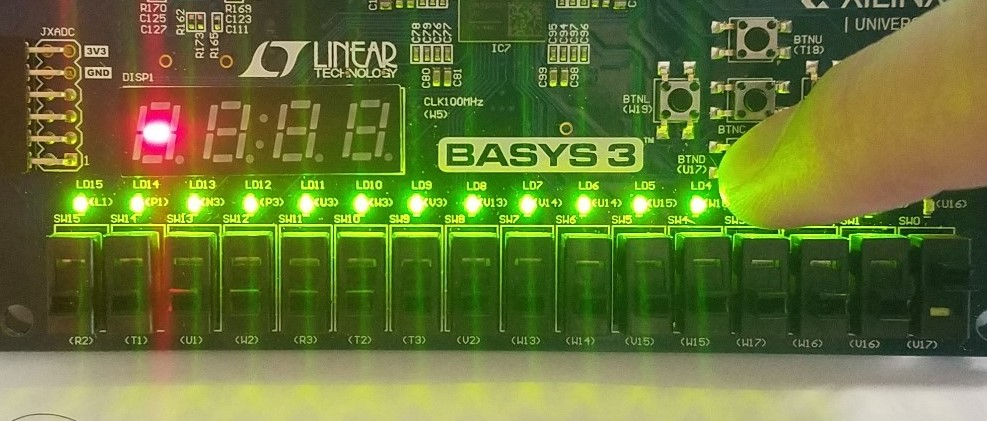
\includegraphics[width=1.0\textwidth,trim=0 0mm 0 0,clip]{Slow3}
\caption{Slow Mode Test 3}
\end{figure}
\begin{figure}[ht]\centering
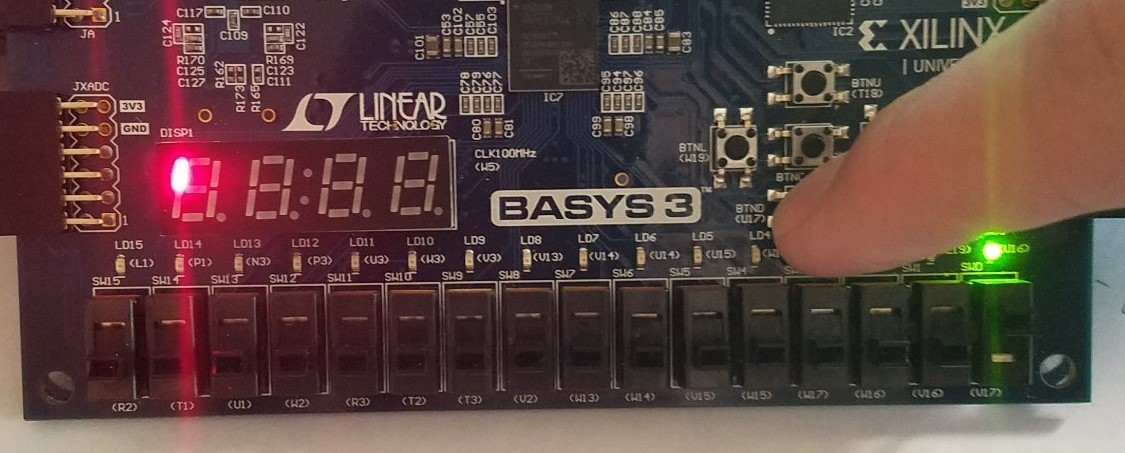
\includegraphics[width=1.0\textwidth,trim=0 0mm 0 0,clip]{Slow4}
\caption{Slow Mode Test 4}
\end{figure}
\begin{figure}[ht]\centering
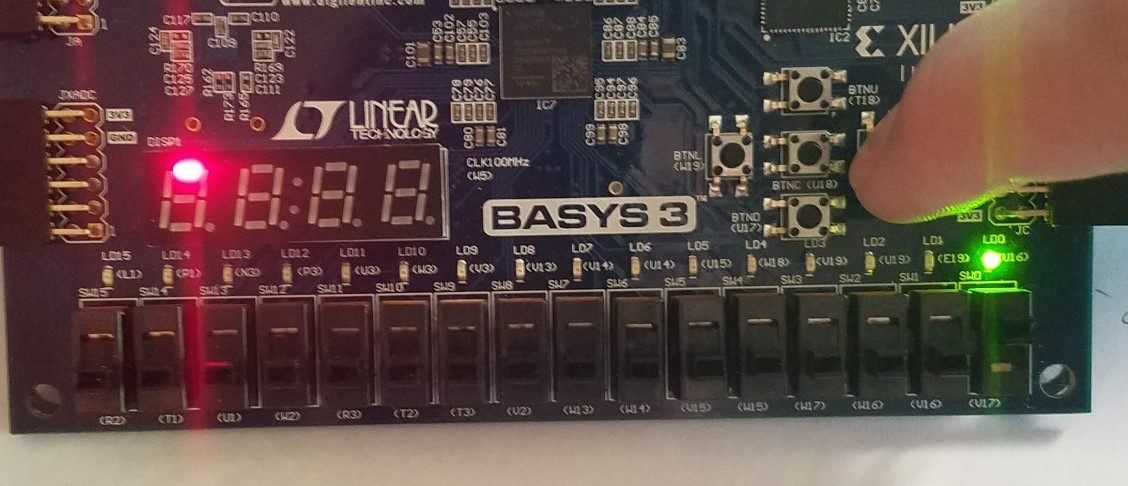
\includegraphics[width=1.0\textwidth,trim=0 0mm 0 0,clip]{Slow5}
\caption{Slow Mode Test 5}
\end{figure}
\begin{figure}[ht]\centering
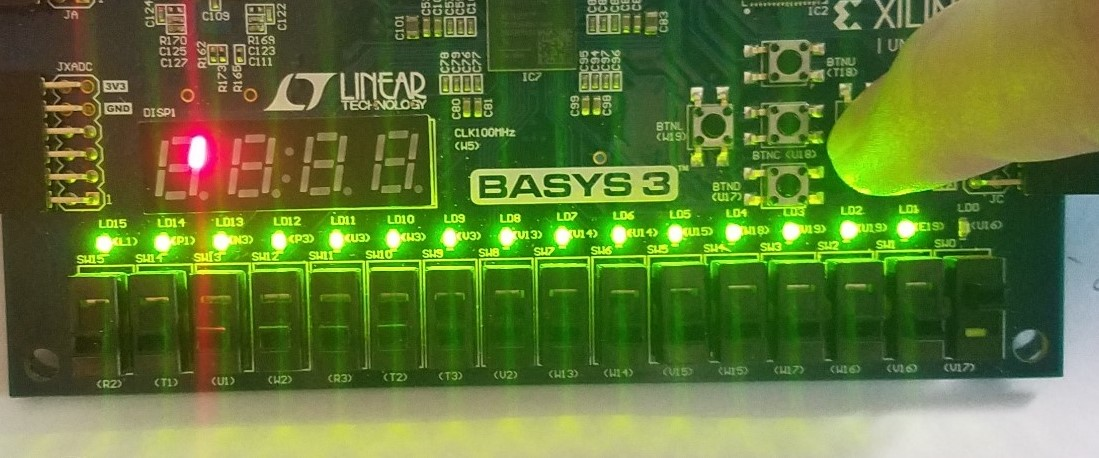
\includegraphics[width=1.0\textwidth,trim=0 0mm 0 0,clip]{Slow6}
\caption{Slow Mode Test 6}
\end{figure}
\begin{figure}[ht]\centering
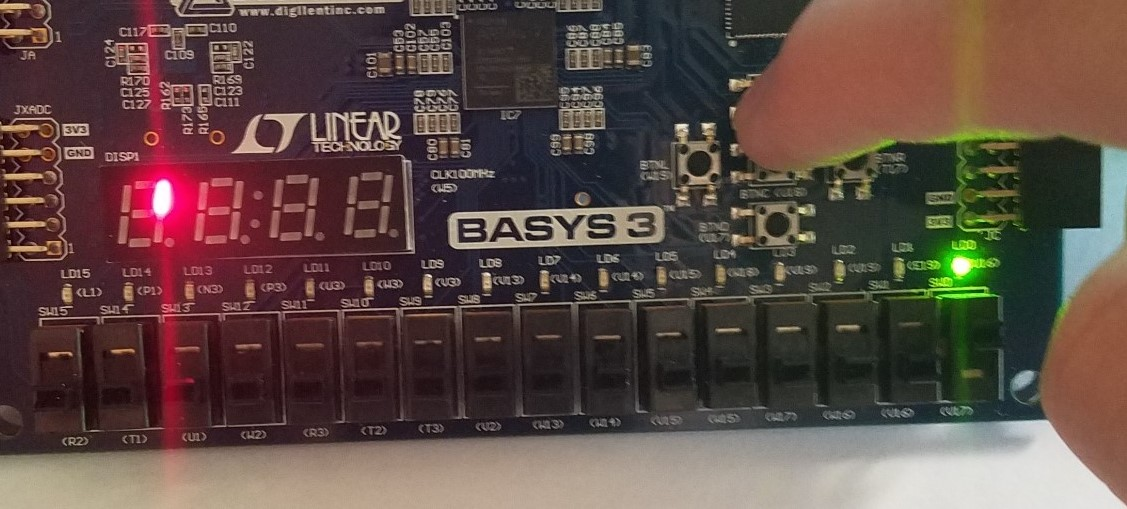
\includegraphics[width=1.0\textwidth,trim=0 0mm 0 0,clip]{Slow7}
\caption{Slow Mode Test 7}
\end{figure}
\begin{figure}[ht]\centering
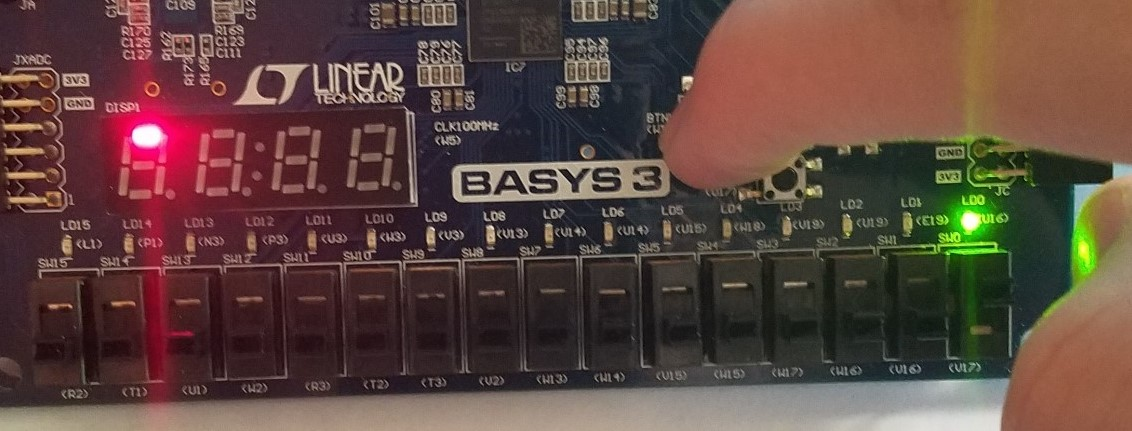
\includegraphics[width=1.0\textwidth,trim=0 0mm 0 0,clip]{Slow8}
\caption{Slow Mode Test 8}
\end{figure}
\begin{figure}[ht]\centering
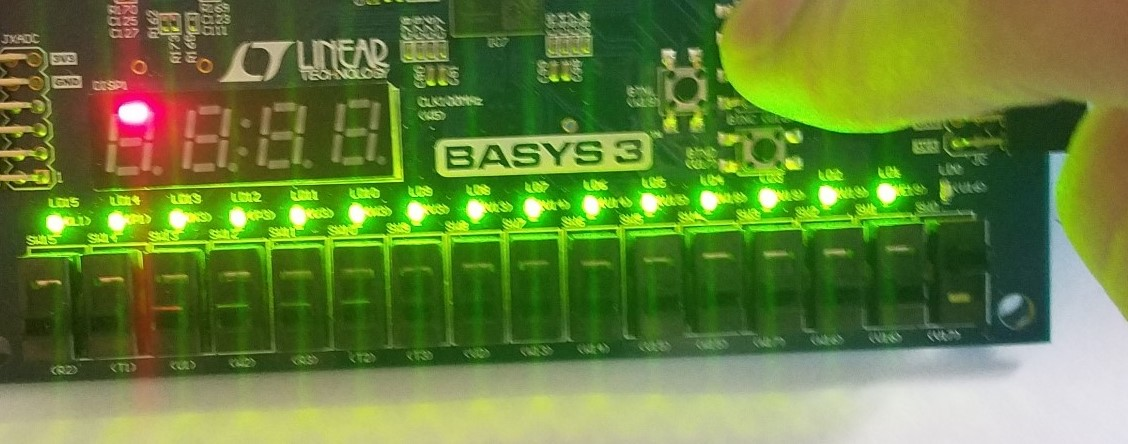
\includegraphics[width=1.0\textwidth,trim=0 0mm 0 0,clip]{Slow9}
\caption{Slow Mode Test 9}
\end{figure}
\begin{figure}[ht]\centering
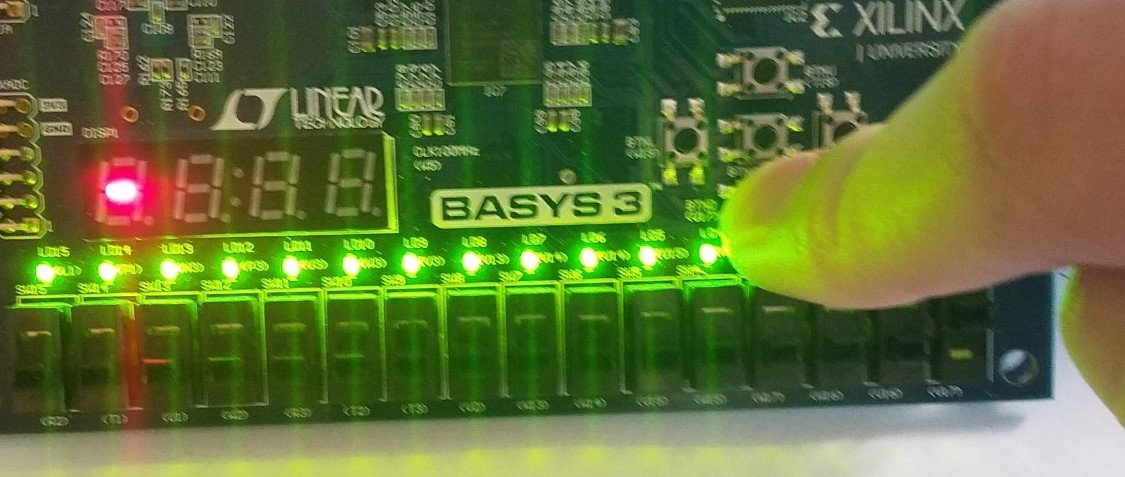
\includegraphics[width=1.0\textwidth,trim=0 0mm 0 0,clip]{Slow10}
\caption{Slow Mode Test 10}
\end{figure}

\clearpage

\subsection{Waveforms}

\begin{figure}[ht]\centering
	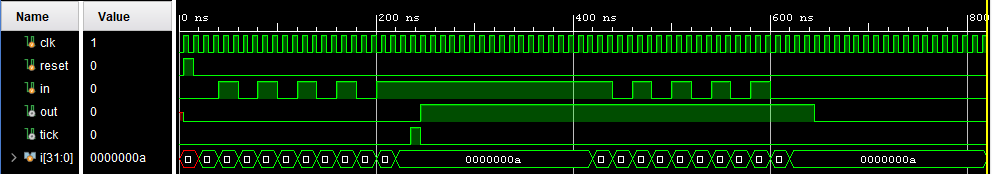
\includegraphics[width=1.0\textwidth,trim=0 0mm 0 0,clip]{Debounce}
	\caption{Debounce Test Waveform}
\end{figure}

\begin{figure}[ht]\centering
	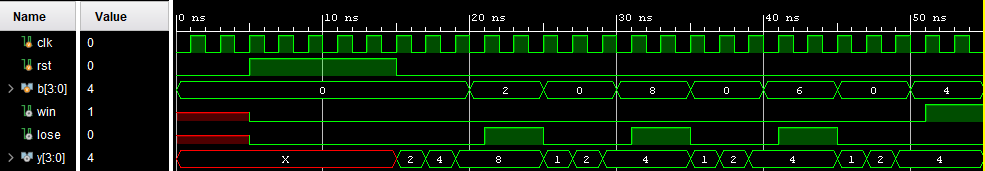
\includegraphics[width=1.0\textwidth,trim=0 0mm 0 0,clip]{FSM}
	\caption{Finite Test Machine Test Waveform}
\end{figure}

\begin{figure}[ht]\centering
	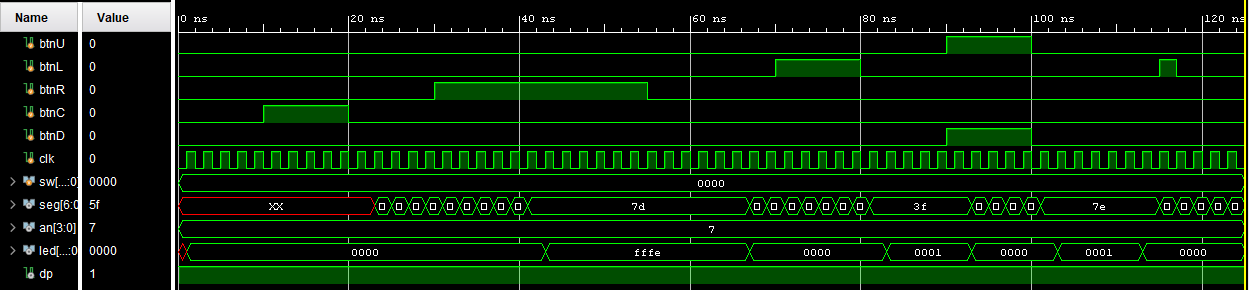
\includegraphics[width=1.0\textwidth,trim=0 0mm 0 0,clip]{GameTest}
	\caption{Game Test Waveform}
\end{figure}

\clearpage

\section*{Code}

\Verilog[firstline=23,caption=Verilog Guessing Game Source,label=code:file_ex]
{guessing_game.sv}

\Verilog[firstline=23,caption=Verilog Guessing Game Test Bench,label=code:file_ex]
{Game_Test.sv}

\Verilog[firstline=23,caption=Verilog Finite State Machine Source,label=code:file_ex]
{guess_FSM.sv}

\Verilog[firstline=23,caption=Verilog Finite State Machine Test Bench,label=code:file_ex]
{guess_Test.sv}





\end{document}
